% Where models help along the research workflow, and the check each stage needs.
% ---------------------------------------------------------------------------
% style.tex --- shared preamble for every figure in book/figures/tikz/
%
% One style for all figures: Latin Modern, thin black lines, a light grey
% fill, and one accent colour used only to mark what is untrusted or wrong.
% Build with scripts/build_figures.sh; see book/figures/README.md.
% ---------------------------------------------------------------------------
\documentclass[tikz,border=6pt]{standalone}
\usepackage[T1]{fontenc}
\usepackage{lmodern}
\usetikzlibrary{arrows.meta,positioning,shapes.geometric,calc,fit,backgrounds}

\hyphenpenalty=10000   % short lines in boxes: ragged, never hyphenated

\definecolor{lightgrey}{gray}{0.92}
\definecolor{accent}{HTML}{9B2D20}

\tikzset{
  every picture/.style={
    line width=0.6pt,
    font=\small,
    >={Stealth[length=5pt,width=4pt]},
    node distance=14pt and 24pt,
  },
  % shapes
  box/.style={draw, rectangle, inner xsep=8pt, inner ysep=5pt,
              minimum height=22pt, align=center},
  grey/.style={box, fill=lightgrey},
  rounded/.style={box, rounded corners=9pt},
  decision/.style={draw, diamond, aspect=2.4, inner sep=1.5pt, align=center},
  group/.style={draw, dashed, rounded corners=5pt, inner sep=7pt},
  % text
  tag/.style={font=\footnotesize, align=center, inner sep=2pt},
  note/.style={font=\footnotesize\itshape, align=center, inner sep=2pt},
  code/.style={font=\small\ttfamily},
  codetag/.style={font=\footnotesize\ttfamily, align=center, inner sep=2pt},
  title/.style={font=\small\scshape, align=center, inner sep=2pt},
  % lines
  arrow/.style={->},
  back/.style={->, dashed},
  thin/.style={line width=0.4pt, gray},
  % the one accent, for what is untrusted, wrong or missing
  bad/.style={accent},
  badbox/.style={box, draw=accent, text=accent},
}

\begin{document}
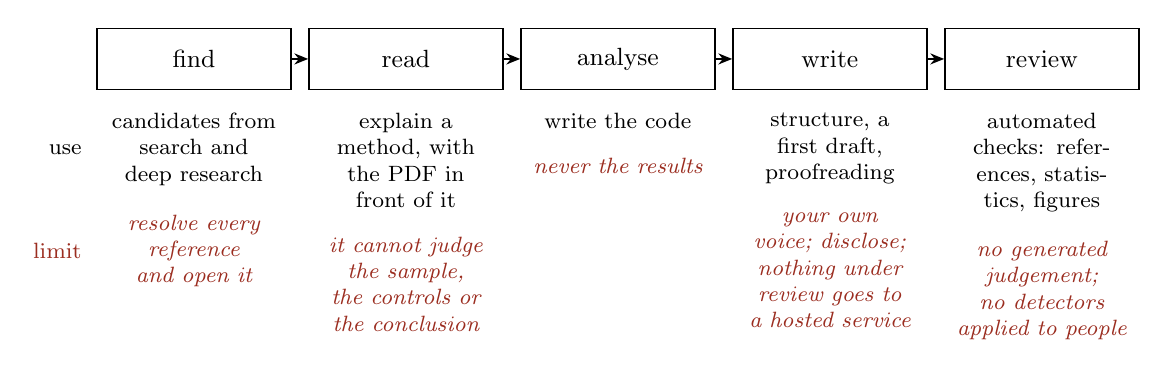
\begin{tikzpicture}[node distance=6pt and 6pt,
                    stage/.style={box, text width=54pt, align=center},
                    use/.style={tag, text width=64pt, align=center},
                    chk/.style={note, text width=64pt, align=center, text=accent}]
  \node[stage] (s1) {find};
  \node[stage, right=of s1] (s2) {read};
  \node[stage, right=of s2] (s3) {analyse};
  \node[stage, right=of s3] (s4) {write};
  \node[stage, right=of s4] (s5) {review};
  \foreach \a/\b in {s1/s2,s2/s3,s3/s4,s4/s5} \draw[->] (\a) -- (\b);
  \node[use, below=of s1] (u1) {candidates from search and deep research};
  \node[use, below=of s2] (u2) {explain a method, with the PDF in front of it};
  \node[use, below=of s3] (u3) {write the code};
  \node[use, below=of s4] (u4) {structure, a first draft, proofreading};
  \node[use, below=of s5] (u5) {automated checks: references, statistics, figures};
  \node[chk, below=of u1] (c1) {resolve every reference and open it};
  \node[chk, below=of u2] (c2) {it cannot judge the sample, the controls or the conclusion};
  \node[chk, below=of u3] (c3) {never the results};
  \node[chk, below=of u4] (c4) {your own voice; disclose; nothing under review goes to a hosted service};
  \node[chk, below=of u5] (c5) {no generated judgement; no detectors applied to people};
  \node[tag, anchor=east, align=right] at ([xshift=-4pt]u1.west) {use};
  \node[tag, anchor=east, align=right, text=accent] at ([xshift=-4pt]c1.west) {limit};
\end{tikzpicture}
\end{document}
